%% This is the ctufit-thesis example file. It is used to produce theses
%% for submission to Czech Technical University, Faculty of Information Technology.
%%
%% This is version 1.3.10, built 27. 2. 2025.
%% 
%% Get the newest version from
%% https://gitlab.fit.cvut.cz/theses-templates/FITthesis-LaTeX
%%
%%
%% Copyright 2024, Tomas Novacek
%% Copyright 2021, Eliska Sestakova and Ondrej Guth
%%
%% This work may be distributed and/or modified under the
%% conditions of the LaTeX Project Public License, either version 1.3
%% of this license or (at your option) any later version.
%% The latest version of this license is in
%%  https://www.latex-project.org/lppl.txt
%% and version 1.3 or later is part of all distributions of LaTeX
%% version 2005/12/01 or later.
%%
%% This work has the LPPL maintenance status `maintained'.
%%
%% The current maintainer of this work is Tomas Novacek.
%% Alternatively, submit bug reports to the tracker at
%% https://gitlab.fit.cvut.cz/theses-templates/FITthesis-LaTeX/issues
%%
%%

% arara: xelatex
% arara: biber
% arara: xelatex
% arara: xelatex

%%%%%%%%%%%%%%%%%%%%%%%%%%%%%%%%%%%%%%%%%
% CLASS OPTIONS
% language: czech/english/slovak
% thesis type: bachelor/master/dissertation
% colour: bw for black&white OR no option for default colour scheme
% electronic (oneside) or printed (twoside), twoside is default
% paragraph - if passed, this optional argument sets paragraphs as the deepest level of headers, styles it, numbers it and adds it to Table of Content. Use with care! Normally, it is considered unwise to use it, since its too deep.
%%%%%%%%%%%%%%%%%%%%%%%%%%%%%%%%%%%%%%%%%
\documentclass[czech,master,unicode,oneside]{ctufit-thesis}

%%%%%%%%%%%%%%%%%%%%%%%%%%%%%%%%%%
% FILL IN THIS INFORMATION
%%%%%%%%%%%%%%%%%%%%%%%%%%%%%%%%%%
\ctufittitle{Porovnání Frama-C a Stainless} % replace with the title of your thesis
\ctufitauthorfull{Bc. Luboš Zápotočný} % replace with your full name (first name(s) and then family name(s) / surname(s)) including academic degrees
\ctufitauthorsurnames{Zápotočný} % replace with your surname(s) / family name(s)
\ctufitauthorgivennames{Luboš} % replace with your first name(s) / given name(s)
\ctufitsupervisor{doc.\,RNDr.\,Dušan Knop,\,Ph.D.} % replace with name of your supervisor/advisor (include academic degrees)
\ctufitdepartment{Katedra teoretické informatiky} % replace with the department of your defence
\ctufityear{2025} % replace with the year of your defence
\ctufitdeclarationplace{Praze} % replace with the place where you sign the declaration
\ctufitdeclarationdate{\today} % replace with the date of signature of the declaration
\ctufitabstractCZE{Fill in the abstract of this thesis in Czech. Lorem ipsum dolor sit amet. Class aptent taciti sociosqu ad litora torquent per conubia nostra, per inceptos hymenaeos. Cras pede libero, dapibus nec, pretium sit amet, tempor quis. Sed vel lectus. Donec odio tempus molestie, porttitor ut, iaculis quis, sem. Suspendisse sagittis ultrices augue.}
\ctufitabstractENG{Fill in the abstract of this thesis in English. Lorem ipsum dolor sit amet. Class aptent taciti sociosqu ad litora torquent per conubia nostra, per inceptos hymenaeos. Cras pede libero, dapibus nec, pretium sit amet, tempor quis. Sed vel lectus. Donec odio tempus molestie, porttitor ut, iaculis quis, sem. Suspendisse sagittis ultrices augue.}
\ctufitkeywordsCZE{enter, comma, separated, list, of, keywords, in, CZECH}
\ctufitkeywordsENG{enter, comma, separated, list, of, keywords, in, ENGLISH}
%%%%%%%%%%%%%%%%%%%%%%%%%%%%%%%%%%
% END FILL IN
%%%%%%%%%%%%%%%%%%%%%%%%%%%%%%%%%%

%%%%%%%%%%%%%%%%%%%%%%%%%%%%%%%%%%
% CUSTOMIZATION of this template
% Skip this part or alter it if you know what you are doing.
%%%%%%%%%%%%%%%%%%%%%%%%%%%%%%%%%%

\RequirePackage{iftex}[2020/03/06]
\iftutex % XeLaTeX and LuaLaTeX
    \RequirePackage{ellipsis}[2020/05/22] %ellipsis workaround for XeLaTeX
\else
    \errmessage{Only compilation with XeLaTeX or LuaLaTeX is allowed}
    \stop
\fi

% hyperlinks
\hypersetup{
    pdfpagelayout=TwoPageRight,
    colorlinks=false,
    allcolors=decoration,
    pdfborder={0 0 0.1}
}

% uncomment the following to hide all hyperlinks
%\hypersetup{hidelinks}

% uncomment the following to change the colour of all hyperlinks to CTU blue
%\hypersetup{allbordercolors=decoration}

\RequirePackage{pdfpages}[2020/01/28]

%%%%%%%%%%%%%%%%%%%%%%%%%%%%%%%%%%
% CUSTOMIZATION of this template END
%%%%%%%%%%%%%%%%%%%%%%%%%%%%%%%%%%


%%%%%%%%%%%%%%%%%%%%%%
% DEMO CONTENTS SETTINGS
% You may choose to modify this part.
%%%%%%%%%%%%%%%%%%%%%%
\usepackage{dirtree}
\usepackage{lipsum,tikz}
\usepackage[style=iso-numeric]{biblatex}
\addbibresource{text/bib-database.bib}
\usepackage{xurl}
\usepackage{listings} % typesetting of sources
\usepackage{minted}
\usepackage{csquotes}

%%%%%%%%%%%%%%%%%%%%%%
% DEMO CONTENTS SETTINGS END
%%%%%%%%%%%%%%%%%%%%%%

\begin{document} 
\frontmatter\frontmatterinit % do not remove these two commands

\thispagestyle{empty}\maketitle\thispagestyle{empty}\cleardoublepage % do not remove these four commands

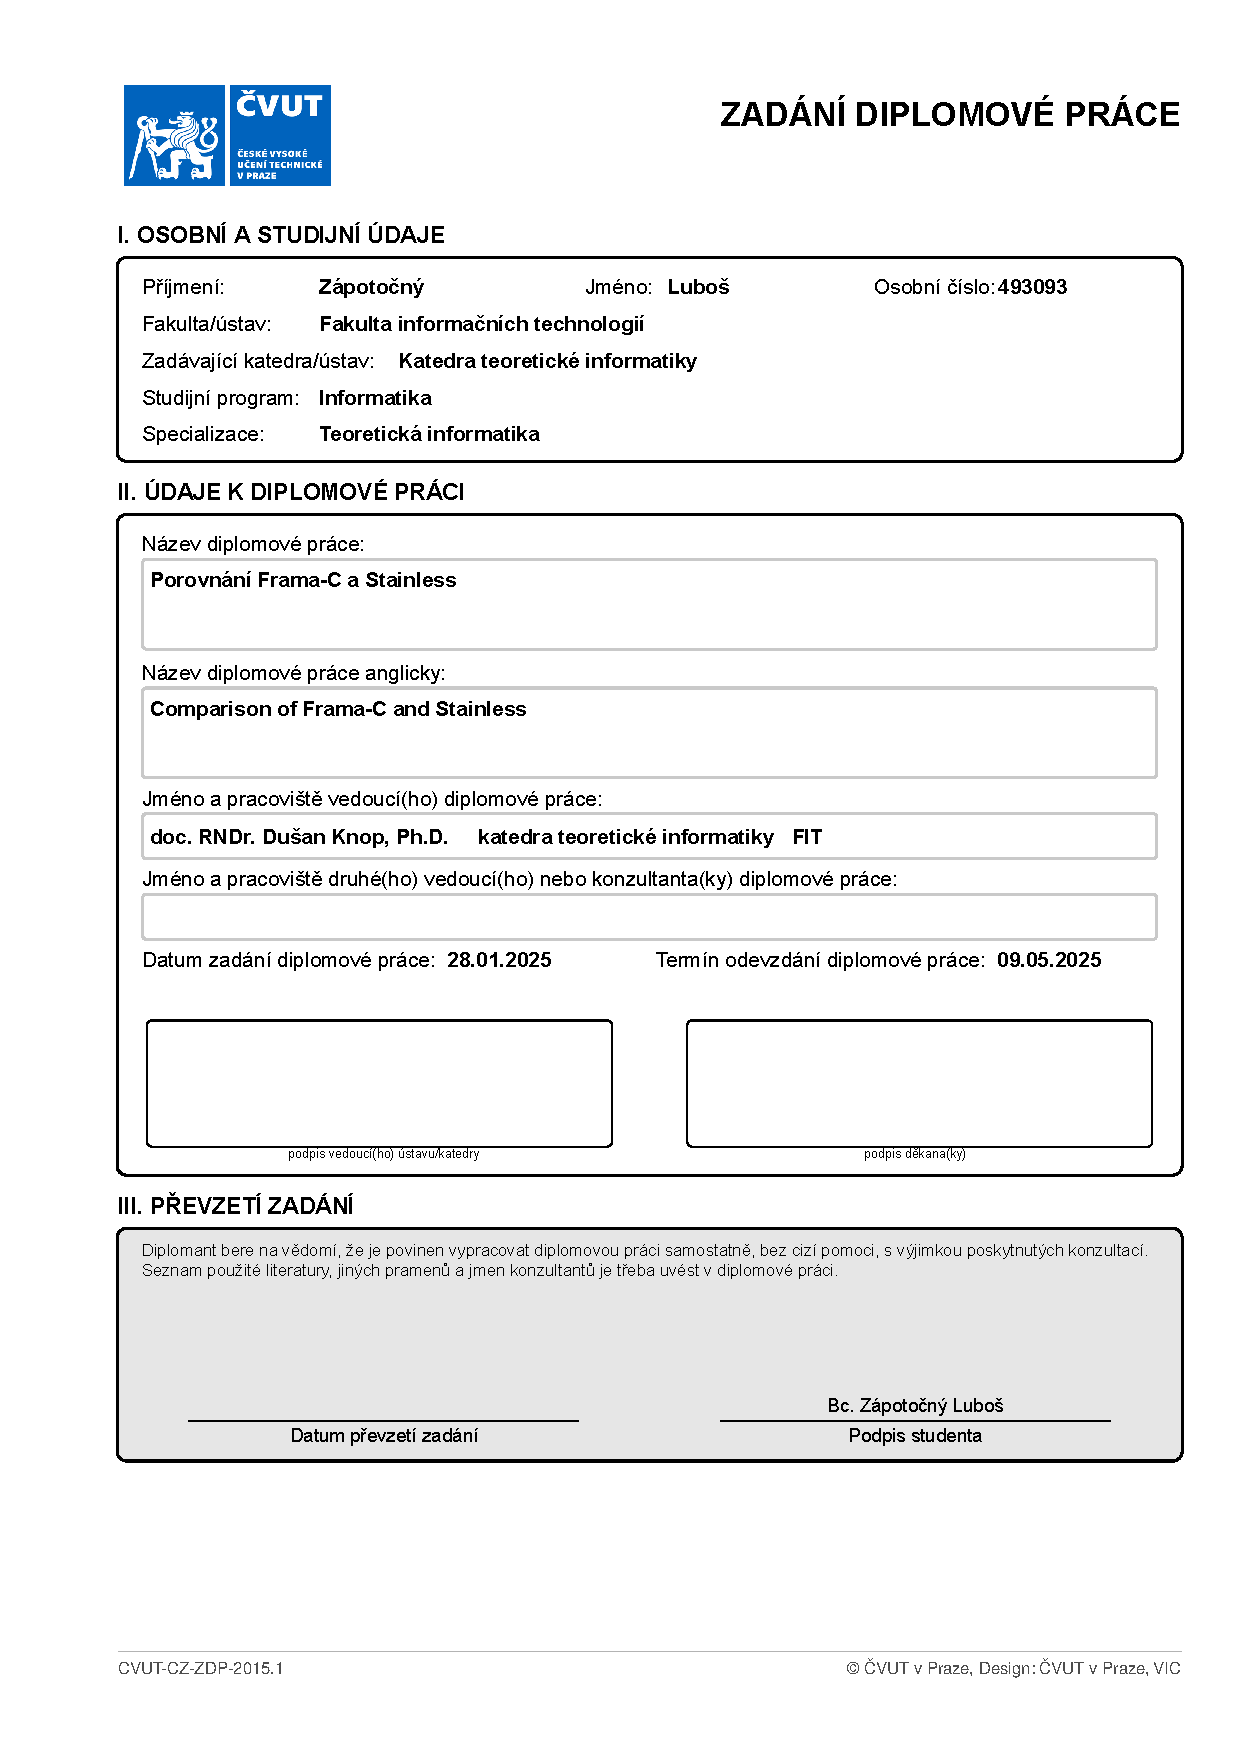
\includepdf[pages={1-}]{zapotlub-assignment.pdf} % replace this file with your thesis assignment generated from ProjectsFIT

\imprintpage % do not remove this command
\stopTOCentries
%%%%%%%%%%%%%%%%%%%%%%
% list of other contents END
%%%%%%%%%%%%%%%%%%%%%%

%%%%%%%%%%%%%%%%%%%
% ACKNOWLEDGMENT
% FILL IN / MODIFY
% This is a place to thank people for helping you. It is common to thank your supervisor.
%%%%%%%%%%%%%%%%%%%
\begin{acknowledgmentpage}
	Chtěl bych poděkovat především sit amet, consectetuer adipiscing elit. Curabitur sagittis hendrerit ante. Class aptent taciti sociosqu ad litora torquent per conubia nostra, per inceptos hymenaeos. Cras pede libero, dapibus nec, pretium sit amet, tempor quis. Sed vel lectus. Donec odio tempus molestie, porttitor ut, iaculis quis, sem. Suspendisse sagittis ultrices augue.
\end{acknowledgmentpage} 
%%%%%%%%%%%%%%%%%%%
% ACKNOWLEDGMENT END
%%%%%%%%%%%%%%%%%%%


%%%%%%%%%%%%%%%%%%%
% DECLARATION
% FILL IN / MODIFY
%%%%%%%%%%%%%%%%%%%
% INSTRUCTIONS
% ENG: choose one of approved texts of the declaration. DO NOT CREATE YOUR OWN. Find the approved texts at https://courses.fit.cvut.cz/SFE/download/index.html#_documents (document Declaration for FT in English)
% CZE/SLO: Vyberte jedno z fakultou schvalenych prohlaseni. NEVKLADEJTE VLASTNI TEXT. Schvalena prohlaseni najdete zde: https://courses.fit.cvut.cz/SZZ/dokumenty/index.html#_dokumenty (prohlášení do ZP)
\begin{declarationpage}
Prohlašuji, že jsem předloženou práci vypracoval samostatně a že jsem uvedl veškeré použité
informační zdroje v souladu s Metodickým pokynem o dodržování etických principů při přípravě
vysokoškolských závěrečných prací.

Beru na vědomí, že se na moji práci vztahují práva a povinnosti vyplývající ze zákona č. 121/2000 Sb.,
autorského zákona, ve znění pozdějších předpisů, zejména skutečnost, že České vysoké učení
technické v Praze má právo na uzavření licenční smlouvy o užití této práce jako školního díla podle §
60 odst. 1 citovaného zákona.
\end{declarationpage}
%%%%%%%%%%%%%%%%%%%
% DECLARATION END
%%%%%%%%%%%%%%%%%%%

\printabstractpage % do not remove this command

%%%%%%%%%%%%%%%%%%%
% SUMMARY
% FILL IN / MODIFY
% OR REMOVE ENTIRELY (upon agreement with your supervisor)
% (appropriate to remove in most theses)
%%%%%%%%%%%%%%%%%%%
% \begin{summarypage}
% \section*{Summary section}
% 
% \lipsum[1][1-8]
% 
% \section*{Summary section}
% 
% \lipsum[2][1-6]
% 
% \section*{Summary section}
% 
% \lipsum[3]
% 
% \section*{Summary section}
% 
% \lipsum[2]
% 
% \section*{Summary section}
% 
% \lipsum[1][1-8] Lorem lorem lorem.
% \end{summarypage}
%%%%%%%%%%%%%%%%%%%
% SUMMARY END
%%%%%%%%%%%%%%%%%%%

\tableofcontents % do not remove this command
%%%%%%%%%%%%%%%%%%%%%%
% list of other contents: figures, tables, code listings, algorithms, etc.
% add/remove commands accordingly
%%%%%%%%%%%%%%%%%%%%%%
\listoffigures % list of figures
\begingroup
\let\clearpage\relax
\listoftables % list of tables
\thectufitlistingscommand
\endgroup

%%%%%%%%%%%%%%%%%%%
% ABBREVIATIONS
% FILL IN / MODIFY
% OR REMOVE ENTIRELY
% List the abbreviations in lexicography order.
%%%%%%%%%%%%%%%%%%%
\chapter{\thectufitabbreviationlabel}
	
\begin{tabular}{rl}
DFA & Deterministic Finite Automaton\\
FA & Finite Automaton\\
LPS & Labelled Prüfer Sequence\\
NFA & Nondeterministic Finite Automaton\\
NPS & Numbered Prüfer Sequence\\
XML & Extensible Markup Language\\
XPath & XML Path Language\\
XSLT & eXtensible Stylesheet Language Transformations\\
W3C & World Wide Web Consortium
\end{tabular}
%%%%%%%%%%%%%%%%%%%
% ABBREVIATIONS END
%%%%%%%%%%%%%%%%%%%
\resumeTOCentries
\mainmatter\mainmatterinit % do not remove these two commands
%%%%%%%%%%%%%%%%%%%
% THE THESIS
% MODIFY ANYTHING BELOW THIS LINE
%%%%%%%%%%%%%%%%%%%

\chapter*{Úvod}
\addcontentsline{toc}{chapter}{Úvod}
\markboth{Úvod}{Úvod}

Tohle je můj úvod práce.

\setcounter{page}{1}

\chapter{Hoareova logika}
\label{ch:hoareova-logika}

Formální systém označovaný jako Hoareova logika byl navržen a popsán
britským matematikem a informatikem C. A. R. Hoarem v roce 1969~\cite{Hoare1969}.
Jedná se o formální systém pro popis a analýzu počítačových programů,
který pro důkaz správnosti programů používá předpoklady (preconditions) a následky (postconditions).

Program popisujeme pomocí Hoareovy trojice

\begin{equation*}
    \{P\} \  Q \  \{R\},
\end{equation*}
kde $P$ jsou předpoklady popisující stav systému před provedením programu,
$Q$ je daný program (příkaz či sekvence příkazů)
a $R$ jsou následky, které popisují stav systému po provedení tohoto programu.
Takto popsaný systém čteme následovně:
\uv{Při splněných předpokladech $P$ budou po provedení programu $Q$ zaručeny následky $R$}.

Hoare v roce 1969 definoval trojici jako $P \ \{ Q \} \  R$,
ale v současnosti se častěji setkáme se zápisem $\{ P \} \  Q \ \{ R \}$.

Předpoklady a následky jsou vyjádřeny jako logické formule,
které popisují vlastnosti proměnných programu v určitém okamžiku.
Následující příklad reprezentuje program, který předpokládá na vstupu nezápornou hodnotu v proměnné $x$
a po provedení programu $Q$ bude zajištěno, že hodnota proměnné $x$ bude kladná (ostře větší než 0).

\begin{equation*}
    \{ x \geq 0 \} \  x \coloneqq x + 1 \  \{ x > 0 \}
\end{equation*}

Předpoklad může být také prázdný, což znamená, že program nevyžaduje žádné speciální podmínky pro spuštění
a formálně tuto situci lze zapsat jako $\{ true \} \  Q \  \{ R \}$.
Pokud je předpoklad prázdný, předpokládáme, že program může být spuštěn
v libovolném stavu systému nebo s libovolnými hodnotami proměnných.
Takový program může vypadat následovně:

\begin{equation*}
    \{ true \} \  x \coloneqq 10 \  \{ x > 0 \}
\end{equation*}

\section{Axiom přiřazení}
\label{sec:hoare-axiom-prirazeni}

Axiom přiřazení je základním pravidlem Hoareovy logiky a nedílnou součástí každého počítačového programu.
Přiřazení je operace obecně zapsaná ve tvaru

\begin{equation*}
    x \coloneqq f,
\end{equation*}
kde $x$ je proměnná a $f$ je výraz bez vedlejších efektů (side effect),
který ale může obsahovat proměnnou $x$, například $x \coloneqq x + 1$.

Chceme zajistit, že jakékoli tvrzení $T$ platné o $f$
je také platné o hodnotě proměnné $x$ po provedení přiřazení.
Označíme si $T[x \leftarrow f]$ tvrzení $T$ ve kterém výskyt proměnné $x$ nahradíme výrazem $f$ (substituce).

Poté můžeme definovat axiom přiřazení jako

\begin{equation*}
    \{ T[x \leftarrow f] \} \  x \coloneqq f \  \{ T \}.
\end{equation*}

Tento zápis říká, že pokud je pravdivé tvrzení $T$, ve kterém
je výskyt proměnné $x$ nahrazen výrazem $f$, pak po provedení přiřazení
je tvrzení $T$ pravdivé také pro proměnnou $x$.
Jedná se tedy o šablonu (schéma) axiomu,
kterou lze použít pro libovolné tvrzení $T$, proměnnou $x$ a výraz $f$.

\section{Pravidlo důsledku}
\label{sec:hoare-pravidlo-dusledku}

Pravidlo důsledku (rule of consequence) je metoda umožnující
tvorbu nových logických tvrzení z již existujících a dokázaných tvrzení.
Základní aplikací této metody je pravidlo \textbf{rozšíření předpokladu}
a pravidlo \textbf{zůžení následku}.
Předpokládejme platnosti $\{ P \} \  Q \  \{ R \}$.

Máme-li rozšířený předpoklad $P'$, pro který platí

\begin{equation*}
    P' \implies P
\end{equation*}
můžeme říci, že

\begin{equation*}
    \{ P' \} \  Q \  \{ R \}
\end{equation*}
je také platné tvrzení.

Máme-li zúžený následek $R'$ následku $R$, pro který platí

\begin{equation*}
    R \implies R'
\end{equation*}
můžeme říci, že $\{ P \} \  Q \  \{ R' \}$ je také platné tvrzení.

\section{Pravidlo skládání}
\label{sec:hoare-pravidlo-skladani}

Pravidlo skládání (rule of composition) je pravidlo, které umožňuje
skládat více příkazů do jednoho složeného příkazu a používat jeje v Hoareově logice.

Máme-li dva příkazy $Q_1$ a $Q_2$, které splňují následující tvrzení

\begin{equation*}
    \{ P_1 \} \  Q_1 \  \{ R_1 \}
\end{equation*}
a

\begin{equation*}
    \{ R_1 \} \  Q_2 \  \{ R_2 \}
\end{equation*}
můžeme říci, že složený příkaz $Q_1; Q_2$ splňuje následující tvrzení

\begin{equation*}
    \{ P_1 \} \  Q_1; Q_2 \  \{ R_2 \}
\end{equation*}
kde $;$ je operátor sekvence příkazů, který říká, že příkaz $Q_1$ bude proveden před příkazem $Q_2$.

Toto pravidlo umožňuje vytvářet složitější příkazy z několika jednodušších příkazů.
Zároveň je možné rozmyslet, že na sekvenci příkazů $Q_1, Q_2, \ldots, Q_n$
lze aplikovat stejné pravidlo skládání, které jsme použili pro dva příkazy
pomocí asociativity operátoru $;$ a závorek. A tedy platí, že

\begin{equation*}
    \{ P \} \  Q_1; Q_2; \  \ldots ; Q_n \  \{ R \}
\end{equation*}
je ekvivalentní s

\begin{equation*}
    \{ P \} \  (Q_1; (Q_2; \  \ldots (Q_{n-1}; Q_n))) \  \{ R \}
\end{equation*}

\section{Pravidlo iterace}
\label{sec:hoare-pravidlo-iterace}

Základním stavebním blokem počítačového programu je cyklus.
V Hoareově logice je cyklus reprezentován pomocí pravidla iterace (rule of iteration)
a využívá $while$ cyklus, který je v programovacích jazycích běžně dostupný a je definován následovně:

\begin{equation*}
    \textbf{while} \  B \  \textbf{do} \  Q
\end{equation*}
kde $Q$ je tělo cyklu, které se v každé iteraci provádí, dokud je podmínka $B$ pravdivá.

Dále definujeme invariant cyklu $I$, který nám pomůže
při rozhodování o správnost cyklu a bude popisovat následky provedení cyklu.
Invariant cyklu je logické tvrzení, které musí být pravdivé před vstupem do cyklu,
po ukončení každé iterace cyklu a tedy i po ukončení cyklu.

Formálně můžeme zapsat podmínky pro invariant cyklu $I$ jako

\begin{equation*}
    I \land (\{ B \} \  Q \  \{ I \})
\end{equation*}

První část konjunkce popisuje, že invariant cyklu musí být pravdivý před vstupem do cyklu.
Druhá část konjunkce popisuje, že invariant cyklu musí být pravdivý po provedení těla cyklu $Q$,
pokud se cyklus spustil (podmínka $B$ byla pravdivá).

\begin{remark}
    Invariant cyklu je nezávislý na počtu provedených iterací.
\end{remark}

Pokud cyklus neprovedl žádnou iteraci a zároveň máme zaručeno,
že invariant cyklu $I$ byl pravdivý před vstupem do cyklu,
triviálně platí, že invariant cyklu $I$ je pravdivý i po ukončení cyklu.
Zároveň platí, že cyklus se neprovedl, protože podmínka $B$ byla nepravdivá.

Pokud cyklus provedl alespoň jednu iteraci a zároveň máme zaručeno,
že invariant cyklu $I$ je pravdivý po ukončení těla cyklu $Q$,
znamená to, že invariant cyklu $I$ je pravdivý i po ukončení poslední iterace cyklu.
Zároven platí, že podmínka $B$ je po ukončení cyklu nepravdivá, jinak by cyklus pokračoval v provádění další iterace.

Formálně lze tedy konstrukci $while$ cyklu pomocí Hoareovy logiky zapsat jako

\begin{equation*}
    I \land \{ B \} \  Q \  \{ I \} \implies \{ I \} \  \textbf{while} \  B \  \textbf{do} \  Q \  \{ \neg B \land I \}
\end{equation*}

\chapter{Metoda nejslabšího předpokladu}
\label{ch:metoda-nejslabsiho-predpokladu}

Metoda nejslabšího předpokladu (weakest precondition, WP) je metoda,
používaná k algoritmickému dokazování správnosti programů pomocí Hoareovy logiky.
Formálně tuto metodu popsal E. W. Dijkstra v roce 1975 a navazuje na práci Hoareho~\cite{Dijkstra1975}.

Připomeneme, že Hoareova trojice je trojice $ \{ P \} \ Q \ \{ R \} $,
kde $P$ je předpoklad, $Q$ je příkaz a $R$ je následek.
Předpoklad $P$ je logický výraz, který musí být pravdivý před provedením příkazu $Q$.
Metoda nejslabšího předpokladu se snaží najít nejslabší předpoklad $WP$, pro který platí

\begin{equation*}
    \{ WP \} \ Q \ \{ R \}
\end{equation*}

a zároveň pro každý jiný předpoklad $P$, pro který by platilo, že

\begin{equation*}
    \{ P \} \ Q \ \{ R \}
\end{equation*}

musí také platit, že

\begin{equation*}
    P \implies WP
\end{equation*}

Tedy, že $WP$ je nejslabší předpoklad pro příkaz $Q$ a následek $R$.

\begin{remark}
    Nejslabší předpoklad $WP$ je (logicky) unikátní pro daný příkaz $Q$ a následek $R$.
\end{remark}

Pokud by existoval jiný kandidát $WP'$ pro nejslabší předpoklad,
poté z definice platí, že

\begin{equation*}
    WP' \implies WP
\end{equation*}

a také, že

\begin{equation*}
    WP \implies WP'
\end{equation*}

Tedy musí platit, že $WP$ a $WP'$ jsou (logicky) ekvivalentní.

Nejslabší předpoklad $WP$ definujeme pomocí transformační funkce $wp$
s parametry $Q$ a $R$ následovně:

\begin{equation*}
    WP = wp(Q, R)
\end{equation*}

Následující kapitoly představují základní pravidla pro algoritmický výpočet nejslabšího předpokladu.
Výpočet začíná vždy od následku $R$ a postupně (od konce k začátku)
analyzuje příkazy $Q_n, Q_{n-1}, \cdots, Q_1$ a aplikuje na ně specifická pravidla.
Výsledkem je nejslabší předpoklad $WP$ pro sekvenci příkazů $Q_1; Q_2; \cdots; Q_n$,
který následně použijeme pro formální důkaz správnosti programu.

\section{Pravidlo přiřazení}
\label{sec:pravidlo-prirazeni}

Výpočet nejslabšího předpokladu pro přiřazení proměnné $x$ hodnoty $E$ je
definován následovně:

\begin{equation*}
    wp(x \coloneqq E, R) = R[x \mapsto E]
\end{equation*}

kde $R[x \mapsto E]$ je substituce výsktytu proměnné $x$ hodnotou $E$ v $R$.

Například pro příkaz $x \coloneqq x + 3$ a následek $x > 0$ dostáváme:

\begin{align*}
    wp(x \coloneqq x + 3, x > 0) & = \\
                                 & = x + 3 > 0 \\
                                 & = x > -3
\end{align*}

Nejslabší předpoklad pro příkaz $x \coloneqq x + 3$, který zaručuje, že
následek $x > 0$ bude pravdivý, je tedy $x > -3$.

\section{Pravidlo sekvence}
\label{sec:pravidlo-sekvence}

Pravidlo sekvence napomáhá k určení nejslabšího předpokladu pro sekvenci příkazů.
Máme-li dva příkazy $Q_1$ a $Q_2$, které splňují následující tvrzení

\begin{equation*}
    \{ P_1 \} \  Q_1 \  \{ R_1 \}
\end{equation*}

a

\begin{equation*}
    \{ R_1 \} \  Q_2 \  \{ R_2 \}
\end{equation*}

můžeme říci, že nejslabší předpoklad pro sekvenci příkazů $Q_1; Q_2$ je

\begin{equation*}
    wp(Q_1; Q_2, R) = wp(Q_1, wp(Q_2, R))
\end{equation*}

Podobně jako v pravidle skládání u Hoareovy logiky z kapitoly~\ref{sec:hoare-pravidlo-skladani}
můžeme rozmyslet výpočet nejslabšího předpokladu pro sekvenci příkazů $Q_1, Q_2, \cdots, Q_n$
pomocí asociativity operátoru $;$ a rekurzivního výpočtu nejslabšího předpokladu.

Například pro příkaz $x \coloneqq x + 3; y \coloneqq x + 2$ a následek $y > 0$ dostáváme:

\begin{align*}
    wp(x \coloneqq x + 3; y \coloneqq x + 2, y > 0) & = \\
                                                     & = wp(x \coloneqq x + 3, wp(y \coloneqq x + 2, y > 0)) \\
                                                     & = wp(x \coloneqq x + 3, x + 2 > 0) \\
                                                     & = x + 3 + 2 > 0 \\
                                                     & = x > -5
\end{align*}

Nejslabší předpoklad pro příkaz $x \coloneqq x + 3; y \coloneqq x + 2$, který zaručuje, že
následek $y > 0$ bude pravdivý, je tedy $x > -5$.

\section{Pravidlo podmínky}
\label{sec:pravidlo-podminky}

Pravidlo podmínky popisuje výpočet nejslabšího předpokladu pro podmínkový příkaz ve tvaru:

\begin{equation*}
    \textbf{if} \ B \ \textbf{then} \ Q_T \ \textbf{else} \ Q_F
\end{equation*}

kde $B$ je podmínka, $Q_T$ je příkaz, který se provede, pokud je podmínka $B$ pravdivá,
a $Q_F$ je příkaz, který se provede, pokud je podmínka $B$ nepravdivá.

Pravidlo podmínky je definováno následovně:

\begin{align*}
    wp(\textbf{if} & \ B \ \textbf{then} \ Q_T \ \textbf{else} \ Q_F, R) = \\
                   & = (B \implies wp(Q_T, R)) \land (\neg B \implies wp(Q_F, R))
\end{align*}

Tedy nejslabší předpoklad pro podmínkový příkaz je logická konjunkce dvou implikací.
Nejslabší předpoklad totiž musí zahrnout oba možné stavy podmínky $B$, případ, kdy je $B$ pravdivá ale také případ, kdy je $B$ nepravdivá.

Pokud je podmínka $B$ pravdivá, použijeme nejslabší předpoklad pro příkaz $Q_T$, tedy $wp(Q_T, R)$.
Pokud není pravdivá ($\neg B$), použijeme nejslabší předpoklad pro příkaz $Q_F$, tedy $wp(Q_F, R)$.

Například pro příkaz $if \ x > 0 \ then \ y \coloneqq x + 3 \ else \ y \coloneqq x - 3$
a následek $y > 0$ dostáváme:

\begin{align*}
    wp(if & \ x > 0 \ then \ y \coloneqq x + 3 \ else \ y \coloneqq x - 3, y > 0) = \\
          & = (x > 0 \implies wp(y \coloneqq x + 3, y > 0)) \land (\neg (x > 0) \implies wp(y \coloneqq x - 3, y > 0)) \\
          & = (x > 0 \implies x + 3 > 0) \land (\neg (x > 0) \implies x - 3 > 0) \\
          & = (x > 0 \implies x > -3) \land (\neg (x > 0) \implies x > 3)
\end{align*}

Použitím pravidla implikace

\begin{align*}
    (P \implies A) \land (\neg P \implies B) & \iff (P \land A) \lor (\neg P \land B)
\end{align*}

můžeme původní výraz zjednodušit následovně:

\begin{align*}
    (x > 0 & \implies x > -3) \land (\neg (x > 0) \implies x > 3) = \\
           & = (x > 0 \land x > -3) \lor (\neg (x > 0) \land x > 3) \\
           & = (x > 0 \land x > -3) \lor (x \leq 0 \land x > 3) \\
           & = (x > 0 \land x > -3) \lor (false) \\
           & = x > 0 \land x > -3 \\
           & = x > -3
\end{align*}

Výpočet nejslabšího předpokladu pro příkaz $if \ x > 0 \ then \ y \coloneqq x + 3 \ else \ y \coloneqq x - 3$,
který zaručuje, že následek $y > 0$ bude pravdivý, je tedy $x > -3$.
Poslední zjednodušení je možné provést, protože $x > 0$ je silnější předpoklad než $x > -3$,
platí že $x > 0 \implies x > -3$.

Zároveň jsme při výpočtu zjistili, že negativní část ($else$) podmínky nemá vliv na výpočet nejslabšího předpokladu,
protože neexistuje žádný předpoklad, který by v případě, že $x \leq 0$ a $y \coloneqq x - 3$, zaručoval, že $y > 0$.

% TODO: navazat treba na Frama-c, ze pokud dokazeme takovyto priklad, tak vsechny
% TODO: i nelogicke priklady po tom jsou podminene pravdive, nehlede na to, ze
% TODO: ze nemaji treba splnitelnost = assert \false

\appendix\appendixinit % do not remove these two commands

%\chapter{Nějaká příloha}
%
%
%Sem přijde to, co nepatří do hlavní části.
 % include `appendix.tex' from `text/' subdirectory

\backmatter % do not remove this command

\printbibliography % print out the BibLaTeX-generated bibliography list

\chapter{Obsah příloh}
% Contents of the attachment

	\dirtree{%
		.1 /.
		.2 frama-c.
		.3 snippets/\DTcomment{ukázkové úryvky kódu pro Frama\mbox{-}C}.
		.2 stainless.
		.3 snippets/\DTcomment{ukázkové úryvky kódu pro Stainless}.
		.3 LinkedList.scala\DTcomment{ověřená struktura spojového seznamu}.
		.3 BinarySearchTree.scala\DTcomment{ověřená struktura binárního vyhledávacího stromu}.
		.3 AVLTree.scala\DTcomment{ověřená struktura AVL stromu}.
	}
 % include `medium.tex' from `text/' subdirectory

\end{document}
